%%%%%%%%%%%%%%%%%%%%%%%%%%%%%%%%%%%
% RSC Chemical Science Edge Article --- chelfit (2026-11-14)
%%%%%%%%%%%%%%%%%%%%%%%%%%%%%%%%%%%

\documentclass[twoside,twocolumn,9pt]{article}
\usepackage{extsizes}
\usepackage[super,sort&compress,comma]{natbib}
\usepackage[version=3]{mhchem}
\usepackage[a4paper, left=1.5cm, right=1.5cm, top=1.785cm, bottom=2.0cm]{geometry}
\usepackage{balance}
\usepackage{mathptmx}
\usepackage{sectsty}
\usepackage{graphicx}
\usepackage{lastpage}
\usepackage[format=plain,justification=justified,singlelinecheck=false,font={stretch=1.125,small,sf},labelfont=bf,labelsep=space]{caption}
\usepackage{float}
\usepackage{fancyhdr}
\usepackage{fnpos}
\usepackage[english]{babel}
\addto{\captionsenglish}{\renewcommand{\refname}{Notes and references}}
\usepackage{array}
\IfFileExists{droidsans.sty}{\usepackage{droidsans}}{\usepackage{helvet}} % fallback if droidsans absent
\usepackage{charter}
\usepackage[T1]{fontenc}
\usepackage[usenames,dvipsnames]{xcolor}
\usepackage{setspace}
\usepackage[compact]{titlesec}
\PassOptionsToPackage{breaklinks=true,colorlinks=false}{hyperref}
\usepackage{hyperref}
\usepackage[utf8]{inputenc}
\usepackage{amsmath,amssymb,booktabs,multirow}
\usepackage{siunitx,url}
\usepackage{epstopdf,tabularx}
\setlength{\emergencystretch}{4em}
\hyphenation{che-la-tor che-late ra-dio-me-tal con-ju-gate trans-fer-able}


\definecolor{cream}{RGB}{222,217,201}


\begin{document}
\pagestyle{fancy}
\thispagestyle{plain}
\fancypagestyle{plain}{\renewcommand{\headrulewidth}{0pt}}

\makeFNbottom
\makeatletter
\renewcommand\LARGE{\@setfontsize\LARGE{15pt}{17}}
\renewcommand\Large{\@setfontsize\Large{12pt}{14}}
\renewcommand\large{\@setfontsize\large{10pt}{12}}
\renewcommand\footnotesize{\@setfontsize\footnotesize{7pt}{10}}
\makeatother

\renewcommand{\thefootnote}{\fnsymbol{footnote}}
\renewcommand\footnoterule{\vspace*{1pt}\color{cream}\hrule width 3.5in height 0.4pt \color{black}\vspace*{5pt}}
\setcounter{secnumdepth}{5}
\makeatletter
\renewcommand\@biblabel[1]{#1}
\renewcommand\@makefntext[1]{\noindent\makebox[0pt][r]{\@thefnmark\,}#1}
\makeatother
\renewcommand{\figurename}{\small{Fig.}~}
\sectionfont{\sffamily\Large}
\subsectionfont{\normalsize}
\subsubsectionfont{\bf}
\setstretch{1.125}
\setlength{\skip\footins}{0.8cm}
\setlength{\footnotesep}{0.25cm}
\setlength{\jot}{10pt}
\titlespacing*{\section}{0pt}{4pt}{4pt}
\titlespacing*{\subsection}{0pt}{15pt}{1pt}

\fancyfoot{}
\fancyfoot[LO,RE]{\vspace{-7.1pt}
\includegraphics[height=9pt]{head_foot/LF}}
\fancyfoot[CO]{\vspace{-7.1pt}\hspace{13.2cm}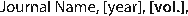
\includegraphics{head_foot/RF}}
\fancyfoot[CE]{\vspace{-7.2pt}\hspace{-14.2cm}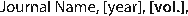
\includegraphics{head_foot/RF}}
\fancyfoot[RO]{\footnotesize{\sffamily{1--\pageref{LastPage} ~\textbar  \hspace{2pt}\thepage}}}
\fancyfoot[LE]{\footnotesize{\sffamily{\thepage~\textbar\hspace{3.45cm} 1--\pageref{LastPage}}}}
\fancyhead{}
\renewcommand{\headrulewidth}{0pt}
\renewcommand{\footrulewidth}{0pt}
\setlength{\arrayrulewidth}{1pt}
\setlength{\columnsep}{6.5mm}
\setlength\bibsep{1pt}

\makeatletter
\newlength{\figrulesep}
\setlength{\figrulesep}{0.5\textfloatsep}
\newcommand{\topfigrule}{\vspace*{-1pt}\noindent{\color{cream}\rule[-\figrulesep]{\columnwidth}{1.5pt}} }
\newcommand{\botfigrule}{\vspace*{-2pt}\noindent{\color{cream}\rule[\figrulesep]{\columnwidth}{1.5pt}} }
\newcommand{\dblfigrule}{\vspace*{-1pt}\noindent{\color{cream}\rule[-\figrulesep]{\textwidth}{1.5pt}} }
\makeatother

%%%%%%%%%%%%%%%%%%%%%%%%%%%%%%%%%%%%%%%%%%%%%%%%%%%%%%%%%%%%%%%%%%%%%%%%%
%%%%%%%%%%%%%%%%%%%%%%%%%%%%%%%%%%%%%%%%%%%%%%%%%%%%%%%%%%%%%%%%%%%%%%%%%
%%%TITLE, AUTHORS AND ABSTRACT%%%
\twocolumn[
  \begin{@twocolumnfalse}
{
\includegraphics[height=30pt]{head_foot/journal_name}\hfill\raisebox{0pt}[0pt][0pt]{
\includegraphics[height=55pt]{head_foot/RSC_LOGO_CMYK}}\\[1ex]

\includegraphics[width=18.5cm]{head_foot/header_bar}}\par
\vspace{1em}
\sffamily
\begin{tabular}{m{4.5cm} p{13.5cm} }


\includegraphics{head_foot/DOI} & \noindent\LARGE{\textbf{A metal chelate's effect on molecular recognition is not a property of the chelate}} \\
\vspace{0.3cm} & \vspace{0.3cm} \\

 & \noindent\large{Jeongyun Kim,$^{\ddag}$\textit{$^{a}$} Jin Yoo,$^{\ddag}$\textit{$^{a}$} Ku Kang$^{\ast}$\textit{$^{a}$} and Dongyoul Lee$^{\ast}$\textit{$^{b}$}} \\

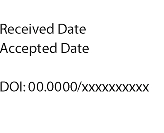
\includegraphics{head_foot/dates} & \noindent\normalsize{\sloppy\setlength{\emergencystretch}{6em}\textbf{Appending a metal chelate to a molecule that binds a biological target changes how tightly it binds. Whether that change is a property of the chelate---and therefore transferable between molecules---is assumed rather than tested, yet it is load-bearing: chelators are chosen from published comparisons and from heuristic metal--chelator matching tables. We audited it. From ten studies we assembled 106 matched affinity measurements in which one targeting molecule was conjugated to two or more chelators and assayed under a single protocol, giving 32 matched sets across five target families. Within a set the chelator alone shifts affinity by a median factor of 2.6 and by up to 25.3, while propagated measurement error accounts for only 11\% of the within-set variance. None of that signal transfers. Under leave-one-target-family-out validation an empirical chelator ranking ($R^2 = -0.250$), classical descriptors ($R^2 = -0.219$) and solvated GFN2-xTB descriptors on 27 structurally verified complexes ($R^2 = -0.340$) all do worse than assuming no effect; none orders a held-out set better than chance, and a within-set permutation test places all of them inside the no-information null. Improving the physics makes this worse rather than better: across a $2\times2$ comparison of energy term and solvation, every step that raises in-sample fit ($R^2 = 0.070 \rightarrow 0.139$) lowers held-out performance ($-0.227 \rightarrow -0.340$). Reported lipophilicity explains 7\% of the effect. What the data do contain is interaction: chelator identity crossed with target family explains $R^2 = 0.498$ against $R^2 = 0.133$ for the chelator alone. The effect is real and large but is not encoded in the chelate; it arises at a contact the isolated complex never makes. We release the dataset, geometries and analysis as an open benchmark.}}\\
\end{tabular}
 \end{@twocolumnfalse} \vspace{0.6cm}
  ]

\renewcommand*\rmdefault{bch}\normalfont\upshape
\rmfamily
\section*{}
\vspace{-1cm}

\footnotetext{\textit{$^{a}$~CBRN Defense Research Institute, Ministry of National Defense, Seoul 06796, Republic of Korea; E-mail: bisu9082@gmail.com}}
\footnotetext{\textit{$^{b}$~Korea Military Academy, Seoul 01805, Republic of Korea; E-mail: [to be supplied]}}
\footnotetext{\ddag~These authors contributed equally.}
\footnotetext{\dag~Electronic Supplementary Information (ESI) available: the matched affinity dataset with per-row DOI provenance, optimised Cartesian geometries of all 32 metal--chelate complexes, the screened candidate pool, and the complete analysis pipeline. See DOI: \texttt{10.5281/zenodo.24211564}.}
%%============================================================
\section{Introduction}
%%============================================================

Coordination chemistry is routinely bolted onto molecular recognition. A metal complex is appended to a molecule that recognises a biological target, and the resulting conjugate is expected to do two jobs at once: hold the metal, and still bind. The design logic that follows treats these jobs as separable---the complex is chosen for its coordination chemistry, and the recognition element for its affinity, as though the first were invisible to the second.

Throughout this article we use \textbf{chelate--vector coupling} for the quantity under study: the change in a conjugate's affinity for its target that follows from changing the chelate alone. This is distinct from \emph{the chelate effect} of classical coordination chemistry, which denotes the enhanced thermodynamic stability of a complex formed by a multidentate rather than monodentate ligand. The two are independent---every complex considered here is a stable chelate in the classical sense, and what varies is what that chelate does to recognition.

Targeted radiopharmaceuticals are where this logic is applied most systematically, and therefore where it can be tested. Radiometal-labelled peptides and protein scaffolds pair a targeting vector with a bifunctional chelator that holds the radiometal, and the chemistry of that chelator has been developed intensively for \ce{^68Ga},\cite{Spang2023GaChelators,Sinnes2020b} for the therapeutic $\alpha$- and $\beta$-emitters now entering the clinic,\cite{Hennrich2026TAT,Mcneil2023Pb} and for large radiometals such as \ce{^227Th} that demand purpose-built cages.\cite{Deberle2025Th227} Purpose-built cages are also the route to stable \ce{^64Cu}/\ce{^67Cu} antibody conjugates, where a sarcophagine replaces the open-chain and macrocyclic chelators that \ce{Cu(ii)} escapes in vivo.\cite{Rudd2025ChemSci} The chelator is usually chosen for radiochemistry---labelling yield, kinetics, and in-vivo complex stability---on the implicit assumption that it is an inert payload holder that does not disturb targeting. Price and Orvig's widely used review codifies that selection logic.\cite{PriceOrvig2014}

That assumption is false, and the field knows it. Fani and co-workers titled their somatostatin study ``The Chelate Makes the Difference'' after finding that swapping the chelator changed receptor affinity substantially.\cite{Fani2011} The same observation has been repeated across essentially every target class that has been examined this way: somatostatin receptor antagonists,\cite{Nicolas2018,Fani2021,Zhang2024JR11} the gastrin-releasing peptide receptor,\cite{Varasteh2015,Abouzayed2019,Guenther2022,Abouzayed2023,Bodei2025,Mitran2016,Mitran2019} CXCR4,\cite{Poschenrieder2016a,Poschenrieder2020,Osl2020} somatostatin-receptor $\alpha$-therapy constructs,\cite{Stallons2022} gastrin and bombesin analogues coupled through different linker chemistries,\cite{Maina2018,Greifenstein2021} and engineered protein scaffolds including affibodies and DARPins.\cite{Rinne2019b,Oroujeni2025,Krasniqi2024}

Every one of these is a one-off empirical comparison: build three or four variants, measure, pick the best. What no study has asked is whether this body of work is cumulative---\textbf{is chelate--vector coupling a property of the chelate?} If a chelator ranking obtained on one vector transfers to another, then a few careful studies could spare the field a great deal of synthesis, and the effect is something a chemist can reason about from the complex. If it does not transfer, then the effect belongs not to the complex but to the pairing, each new construct must be screened from scratch, and published rankings are evidence about nothing but the vector they were measured on.

There is good reason to expect the optimistic answer, and we have ourselves argued for it. Density functional calculations on DOTA, NOTA, NODAGA and TETA complexes reproduce and rationalise the observed ordering of \emph{chelation stability}: cavity volume, ligand rigidity and charge neutrality of the resulting complex together account for which chelator holds which radiometal, and this is enough to rationalise chelator selection on radiochemical grounds.\cite{Kim2026ChelatorDFT} Matched-chelator series on a single vector likewise behave systematically when the readout is radiochemical---the \ce{^212Pb} series on somatostatin-targeting peptides is a case in point.\cite{Kim2026PbSSTR2} The question this article asks is whether the same complex-level reasoning extends from holding the metal to binding the target. These are different physical questions, and a descriptor set that answers the first is not thereby licensed to answer the second.

Prediction of metal--ligand stability constants by machine learning is by now a mature area, but thermodynamic stability is again not the quantity at issue: the constructs being compared all form stable complexes, and the differences appear in recognition. We therefore audited transfer directly, and did so under the validation discipline that the computational chemistry literature has converged on. Random splits inflate apparent performance whenever rows share structure, in some benchmarks by as much as 0.21 in AUC;\cite{Kim2026TAS2R} published benchmarks frequently overstate gains once weak baselines and leakage are controlled for;\cite{McGreivy2024Weak,Schuh2026Audit} and grouped or structure-aware splits are now the recommended default for chemical datasets.\cite{Boldini2025UMAP,Tropsha2025Eval} We adopt a leave-one-target-family-out design for precisely this reason. Because a null result from coarse descriptors would be uninformative, we also computed explicit quantum-chemical descriptors on structurally verified, solvated geometries of each metal--chelate complex, in the spirit of hybrid schemes that feed quantum-chemical quantities into statistical models,\cite{Kang2025QSAR} so that the audit tests the class of complex-level description rather than one careless choice of it.

%%============================================================
\section{Results and discussion}
%%============================================================

\subsection{The effect under audit is large}

Changing only the chelator, with vector, metal and assay fixed, shifts affinity by a median factor of \textbf{2.62}; six of 32 sets exceed fivefold and the largest is \textbf{25.3-fold} (pentixafor with \ce{Cu}: NOTA 46.1\,nM versus DOTAGA 1165\,nM\cite{Poschenrieder2016a}) (Fig.~\ref{fig:1}a). This is not a marginal effect.

\subsection{It is not an artefact of measurement error}

Propagating the reported standard deviations to the log scale gives a median single-measurement error of 0.065 log$_{10}$ units, or 0.092 for a within-set contrast. Measurement error therefore accounts for \textbf{11.0\%} of the within-set variance and genuine signal for \textbf{89.0\%} (Fig.~\ref{fig:1}b). Any descriptor that captured the effect could in principle reach $R^2 = 0.890$.

\subsection{Its direction reverses from one target to the next}

Across 18 matched sets containing both DOTA and NODAGA, DOTA was the stronger binder in 10 and NODAGA in 8 (Fig.~\ref{fig:1}c). For DOTA versus NOTA the split is 8 of 16. The mean contrasts are small and their confidence intervals cross zero: DOTA $-$ NODAGA, $\Delta$log$_{10} = +0.139$, 95\% CI $[-0.042, +0.325]$, $d_z = 0.337$, Wilcoxon $p = 0.265$; DOTA $-$ NOTA, $\Delta$log$_{10} = +0.012$, 95\% CI $[-0.131, +0.167]$, $p = 0.938$. Large per-set effects coexist with no reproducible ordering.

\subsection{No description of the complex survives transfer, quantum chemistry included}

Under leave-one-target-family-out (LOPO) validation---the grouped-split discipline now standard for structurally clustered chemical data\cite{Boldini2025UMAP,Tropsha2025Eval}---on the 82 rows with quantum-chemical coverage (Fig.~\ref{fig:2}a, Table~\ref{tab:lopo}), every model is worse than assuming no effect, and the combined model is worst---the signature of fitting noise. Increasing ridge regularisation improves the quantum-chemical model only by shrinking it toward the zero predictor ($R^2 = -0.453$, $-0.340$, $-0.215$, $-0.111$ at $\alpha = 0.1$, 1, 10, 100), never past it.

\begin{table}[h]
\small
\caption{Leave-one-target-family-out performance ($n = 82$). Confidence intervals are from 10\,000 bootstrap resamples.}
\label{tab:lopo}
\begin{tabular*}{\columnwidth}{@{\extracolsep{\fill}}lrr}
\toprule
Model & LOPO $R^2$ & 95\% CI \\
\midrule
No effect (predict 0)      & $0.000$  & $[-0.064, 0.000]$ \\
Universal chelator ranking & $-0.250$ & $[-0.433, -0.131]$ \\
Classical descriptors      & $-0.219$ & $[-0.391, -0.102]$ \\
GFN2-xTB/ALPB descriptors  & $-0.340$ & $[-0.677, -0.105]$ \\
Classical $+$ quantum      & $-0.480$ & $[-0.915, -0.226]$ \\
\bottomrule
\end{tabular*}
\end{table}

Improving the physics does not help; it hurts, and it does so monotonically. The two improvements we made are separable---replacing the charge-dominated complexation energy with the ligand-exchange energy, and replacing the gas-phase treatment with ALPB solvation---so we ran all four combinations on the same 82 rows (Table~\ref{tab:ladder}). Every step that makes the chemistry more defensible raises the in-sample fit and lowers the held-out performance, on both axes independently and in every ordering. The additional chemical information is real and it is context-specific: it improves the fit where the data are and makes the extrapolation worse. This is the signature of a descriptor set that is learning the dataset rather than the effect, and it is the reason we do not read the in-sample numbers as partial success.

\begin{table}[h]
\small
\caption{Both axes of physical improvement move in-sample fit and held-out performance in opposite directions ($n = 82$ throughout, leave-one-target-family-out).}
\label{tab:ladder}
\begin{tabular*}{\columnwidth}{@{\extracolsep{\fill}}llrr}
\toprule
Energy term & Phase & In-sample $R^2$ & LOPO $R^2$ \\
\midrule
Complexation & gas       & $0.070$ & $-0.227$ \\
Exchange     & gas       & $0.086$ & $-0.280$ \\
Complexation & solvated  & $0.129$ & $-0.328$ \\
Exchange     & solvated  & $0.139$ & $-0.340$ \\
\bottomrule
\end{tabular*}
\end{table}

A within-set permutation test confirms that this is indistinguishable from chance (Fig.~\ref{fig:2}b): the observed solvated result ($R^2 = -0.340$) sits inside the null distribution obtained by shuffling chelator labels within sets (null mean $-0.207$, 95\% interval $[-0.454, -0.004]$, $p = 0.868$), as does the classical result ($R^2 = -0.219$; null mean $-0.145$, $p = 0.766$).

Lipophilicity does not account for the effect either. Across the 29 within-set pairs for which a log$D_{7.4}$ or log$P$ value was reported alongside the affinity, the difference in lipophilicity explains 7.4\% of the difference in affinity and the association is not significant ($r = +0.272$, $p = 0.153$, bootstrap 95\% CI $[-0.146, +0.580]$); the absolute values are uncorrelated ($r = -0.040$, $p = 0.838$).

Transfer fails at every level of generalisation, not only across families (Fig.~\ref{fig:3}b). With the classical descriptors on the full 95 observations, held-out chelator gives $R^2 = -0.020$, held-out vector $-0.088$, held-out paper $-0.086$, held-out target family $-0.177$ and held-out metal $-0.187$; adding the quantum-chemical descriptors on the 82 rows that carry them makes every level worse ($-0.935$, $-0.338$, $-0.344$, $-0.480$ and $-0.137$ respectively). No grouping of the data leaves a positive result anywhere.

\subsection{The descriptors are chemically meaningful, and an apparent signal still fails}

A null result invites the objection that the descriptors were simply poor. They were not. In the space of the twelve descriptors the 32 complexes organise chemically: complexes of the same chelator sit closer together than complexes of different chelators (median pairwise distance 3.92 against 4.65 in the standardised descriptor space; Mann--Whitney $p = 8 \times 10^{-4}$), and the first two principal components, carrying 46\% and 23\% of the variance, separate the macrocyclic cavity sizes and the metal-free ligands (Fig.~\ref{fig:4}a,b). Quantum-chemical quantities of this kind are routinely informative when used as descriptors in statistical models,\cite{Kang2025QSAR} and ours behave accordingly. The ligand-exchange energies order chemically as well: NOTA is destabilised relative to DOTA for every metal ($+14$ to $+21$\,kcal\,mol$^{-1}$) and DOTAGA stabilised ($-6$ to $-36$\,kcal\,mol$^{-1}$), with the larger ions favouring the more donor-rich chelators.

That organisation even produces an apparent relationship with the data, and the fate of that relationship is instructive. Pooling all 95 within-set chelator pairs, the distance between two complexes in descriptor space correlates with the size of the affinity difference between them---larger chemical difference, larger perturbation (Fig.~\ref{fig:4}c). Computed on our first, gas-phase descriptor set the correlation looked solid ($r = +0.326$, $p = 0.001$; Spearman $\rho = +0.241$, $p = 0.019$), and taken at face value it would support a useful rule. Recomputing it on the physically defensible solvated descriptors weakens it to $r = +0.227$ ($p = 0.027$) with a bootstrap 95\% confidence interval that crosses zero, $[-0.088, +0.474]$, and a rank correlation that is no longer significant ($\rho = +0.098$, $p = 0.344$). Nothing about the data changed between those two numbers---only the quality of the physics---and the signal halved.

What remains does not survive validation (Fig.~\ref{fig:4}d). Predicting the magnitude of the effect in a held-out target family gives $R^2 = -0.277$ from the descriptor distance and $R^2 = -0.240$ from the full difference vector. Predicting its \emph{direction} is at chance by construction and in fact: because the ordering within a pair is arbitrary, we evaluated direction on the antisymmetrised pair set, where chance is exactly 0.500, and obtained AUC $= 0.476$ (accuracy 0.511); predicting the signed effect itself gives $R^2 = -0.563$. The pooled correlation with the signed difference is absent to begin with ($r = +0.000$, $p = 0.998$): descriptor distance carries a little information about \emph{how much} a chelator swap moves affinity and none at all about \emph{which way}. The apparent signal is a pooled artefact of exactly the kind this audit was designed to detect, and of the kind that systematic re-examination of published benchmarks repeatedly uncovers.\cite{Schuh2026Audit,McGreivy2024Weak}

\subsection{What the audit would have caught}

Injecting an effect that is by construction a linear function of the descriptors---hence perfectly transferable---gives a detection curve (200 random descriptor directions per magnitude; detection defined as LOPO $R^2 > 0$). The design detects a transferable twofold effect about three times in four (74\%), reaches 80\% only near fourfold, and has essentially no power below 1.4-fold. The observed within-set effects have a median magnitude of 1.50-fold and reach 5.5-fold, so effects of the relevant size exist in the data---they are simply not transferable. A transferable component of twofold or more is excluded with roughly 75\% confidence; a component smaller than ${\sim}1.4$-fold is beyond what this dataset can resolve.

The same conclusion follows from a metric that does not depend on $R^2$ at all. Asked merely to put the chelators of a held-out set in the right order, every model performs at chance: the universal ranking orders 8 of 18 sets correctly (mean $\rho = -0.055$, 95\% CI $[-0.361, +0.261]$), classical descriptors 9 of 18 ($\rho = -0.066$), quantum-chemical descriptors 8 of 18 ($\rho = +0.001$) and their union 9 of 18 ($\rho = -0.005$).

\subsection{The structure is real, and it lives in the pairing}

The failure is not an absence of structure (Fig.~\ref{fig:3}a). Chelator identity alone explains $R^2 = 0.133$ of within-set variance; chelator interacted with target family explains $R^2 = 0.498$---nearly four times as much. By contrast the quantum-chemical descriptors explain only $R^2 = 0.139$ of the within-set variance \emph{in sample}. The information needed to predict the effect is present in the chelator\,$\times$\,vector combination and absent from any property of the isolated complex that we computed.

\subsection{Why a property of the complex cannot carry it}

A metal chelate appended to a targeting molecule is not a spectator. It sits at the conjugation site, usually the vector's N-terminus, close enough to the recognition interface that its steric bulk, charge distribution and rigidity enter the binding event. What it costs there is set by what the receptor presents at that position---and SSTR2, GRPR, CXCR4, PSMA and an engineered scaffold present different things. The somatostatin receptor alone distinguishes agonist from antagonist binding modes sharply enough to change internalisation and tumour uptake,\cite{Zhu2024SSTRanta,Zhang2024JR11} which is the scale of discrimination a chelate at the N-terminus is being asked to be invisible to. The quantity that governs the effect is therefore a contact, and a contact belongs to a pair. No property of the isolated complex, however carefully computed, can encode a partner it never meets.

Read this way the audit does not report a failure of description; it locates the missing information. Charge, denticity, cavity fit, exchange energy, dipole, metal partial charge and coordination geometry are all genuine properties of the complex, and all of them are silent about the pairing. This is not a retraction of complex-level reasoning: the same quantities do account for chelation stability,\cite{Kim2026ChelatorDFT} and the present result delimits their reach rather than denying it. The quantum-chemical arm matters precisely because it rules out the easy explanation: the descriptors were not crude, the geometries were solvated and verified against known coordination modes, and they still carry nothing transferable.

The practical consequence is direct. A published statement that chelator X outperforms chelator Y is evidence about the vector it was measured on and should not be carried to a new construct; our data show the ordering is as likely to reverse as to hold. Chelator screening cannot be replaced by literature-based selection or by computational pre-screening with complex-level descriptors, and should be treated as a required experimental step for each new vector. Reporting a full matched series rather than only the winning variant therefore has unusual value, since only matched series support this kind of analysis; studies that publish the complete series on one vector\cite{Kim2026PbSSTR2,Guenther2022,Abouzayed2023} are the ones this analysis could use at all. The same argument applies to any affinity-based computational pre-screen, whose reported accuracy likewise depends on how its evaluation sets were constructed.\cite{Kang2026Docking,Kang2026GasBench}

\subsection{Limitations}

The dataset is small---95 matched-set observations in 32 sets across five target families---and LOPO with five folds is a demanding test. We regard the alternative as worse: a random split over matched sets would have reported a confident positive result, which is the failure mode grouped validation exists to prevent.\cite{Kim2026TAS2R,Boldini2025UMAP} We have quantified rather than merely acknowledged this: the injection analysis resolves transferable effects of twofold and above about three times in four and is blind below roughly 1.4-fold, and because the injected effect was linear in the descriptors, the easiest case to learn, that floor is optimistic. The five target families span peptides and engineered protein scaffolds, which differ in how far the chelate sits from the binding interface; the direction reversals nonetheless occur within the peptide families alone. Endpoints were pooled across IC$_{50}$, $K_\text{i}$ and $K_\text{D}$; within-set centring makes this defensible---no set mixes endpoints---but it assumes chelate--vector coupling acts comparably on all three. Three of the ten studies come from two laboratories. Thirteen values involving AAZTA5, benzyl-substituted chelators and the [\ce{AlF}]$^{2+}$ unit lacked quantum-chemical descriptors and were excluded from those models while retained in the descriptive analyses.

%%============================================================
\section{Conclusions}
%%============================================================

We audited a load-bearing assumption of conjugate design: that the effect a metal chelate has on molecular recognition is a property of the chelate. Across ten studies and 106 matched affinity measurements the effect is unambiguous---chelator choice alone moves affinity by a median factor of 2.6 and by up to 25-fold, with measurement error accounting for only 11\% of the within-set variance. It is also unambiguously non-transferable. No empirical ranking, no classical physicochemical descriptor set, and no solvated GFN2-xTB descriptor set computed on structurally verified geometries predicts the effect in a held-out target family; all do worse than assuming no effect, none is separable from a within-set permutation null, and none orders held-out chelators better than chance. An injection analysis bounds the claim: a transferable component of twofold or more would have been caught three times in four. What the data do contain is interaction---chelator identity crossed with target family explains 50\% of within-set variance against 13\% for the chelator alone.

Chelate--vector coupling is therefore not a property of the chelate but of the pairing, and it must be measured in each pairing. For practice this reverses the usual inference: a published chelator comparison is evidence about the vector it was measured on. For description it says where to look next---not at better properties of the complex, but at the complex in contact with its target.

\begin{figure}[t]
\centering
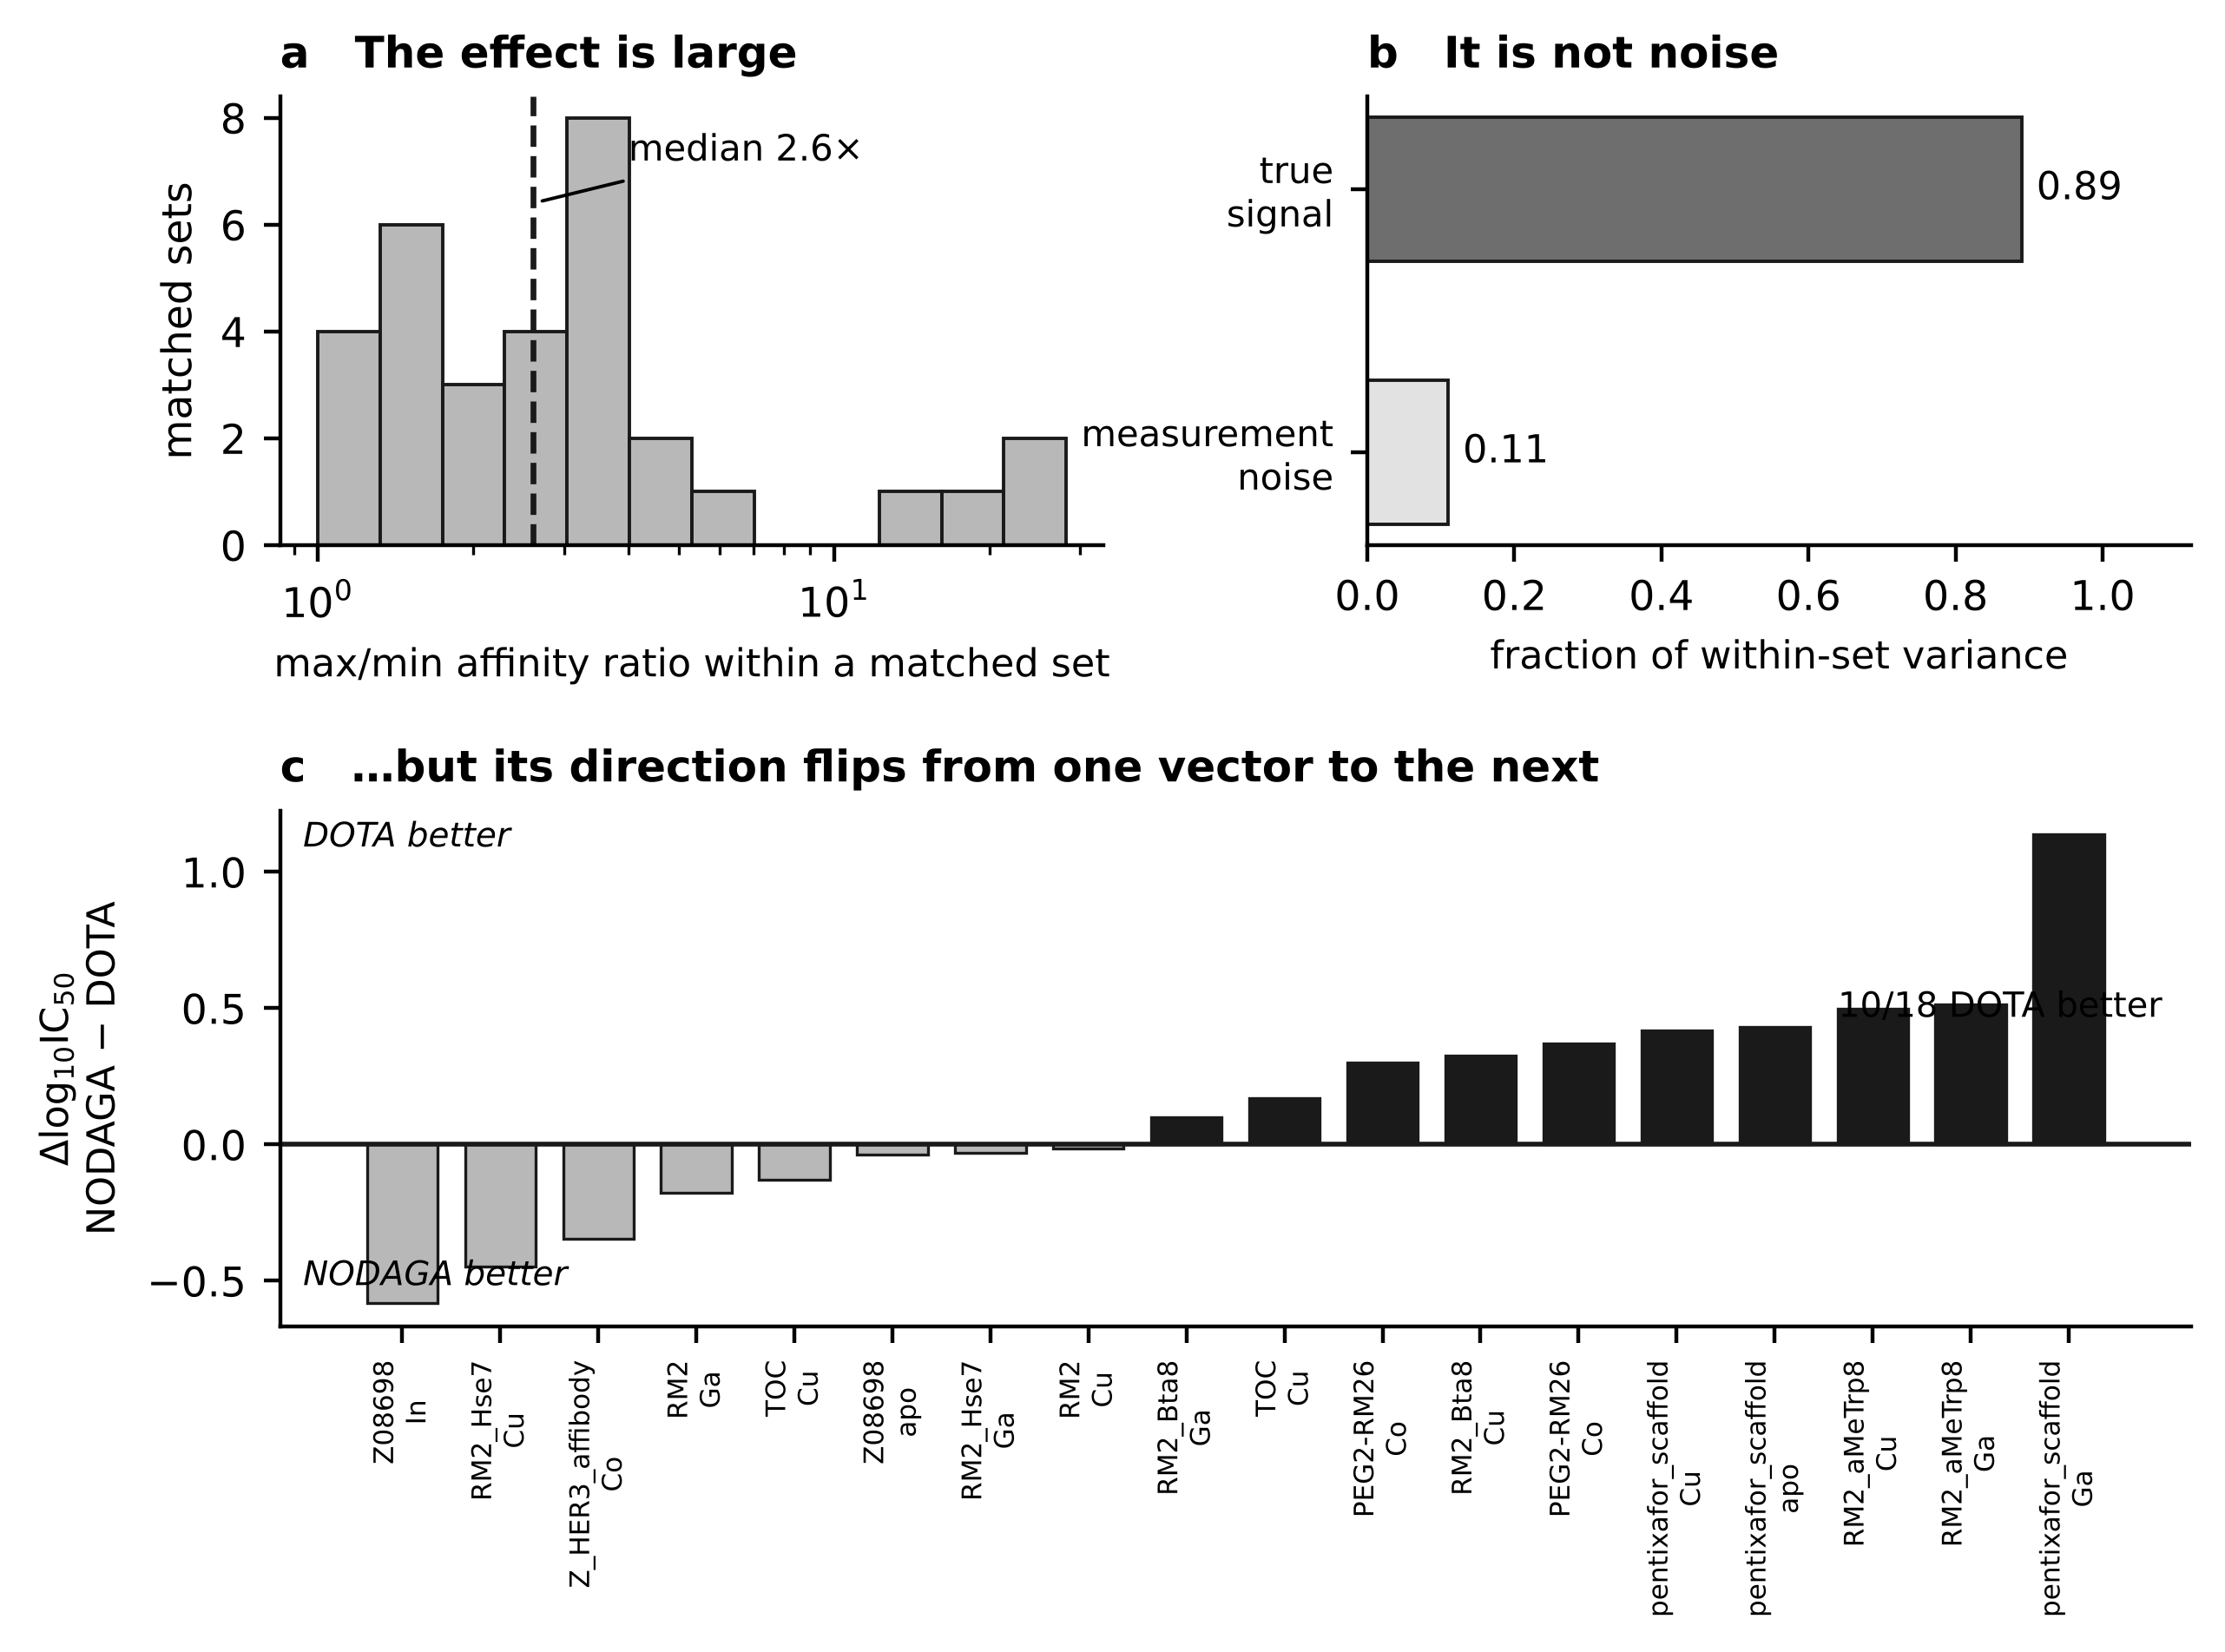
\includegraphics[width=\columnwidth]{Fig1.png}
\caption{\textbf{Chelate--vector coupling is large, is not noise, and reverses between vectors.} (\textbf{a}) Distribution of the maximum/minimum affinity ratio within each of 32 matched sets; dashed line, median 2.6-fold. (\textbf{b}) Decomposition of within-set variance into measurement error, propagated from reported standard deviations, and true signal. (\textbf{c}) Within-set difference in log$_{10}$ affinity between DOTA and NODAGA for all 18 sets containing both, labelled by vector and metal; bars above zero (green) mark sets in which NODAGA is the stronger binder, bars below zero (orange) those in which DOTA is. The direction reverses from one vector to the next, 8 of 18 favouring NODAGA.}
\label{fig:1}
\end{figure}

\begin{figure}[t]
\centering
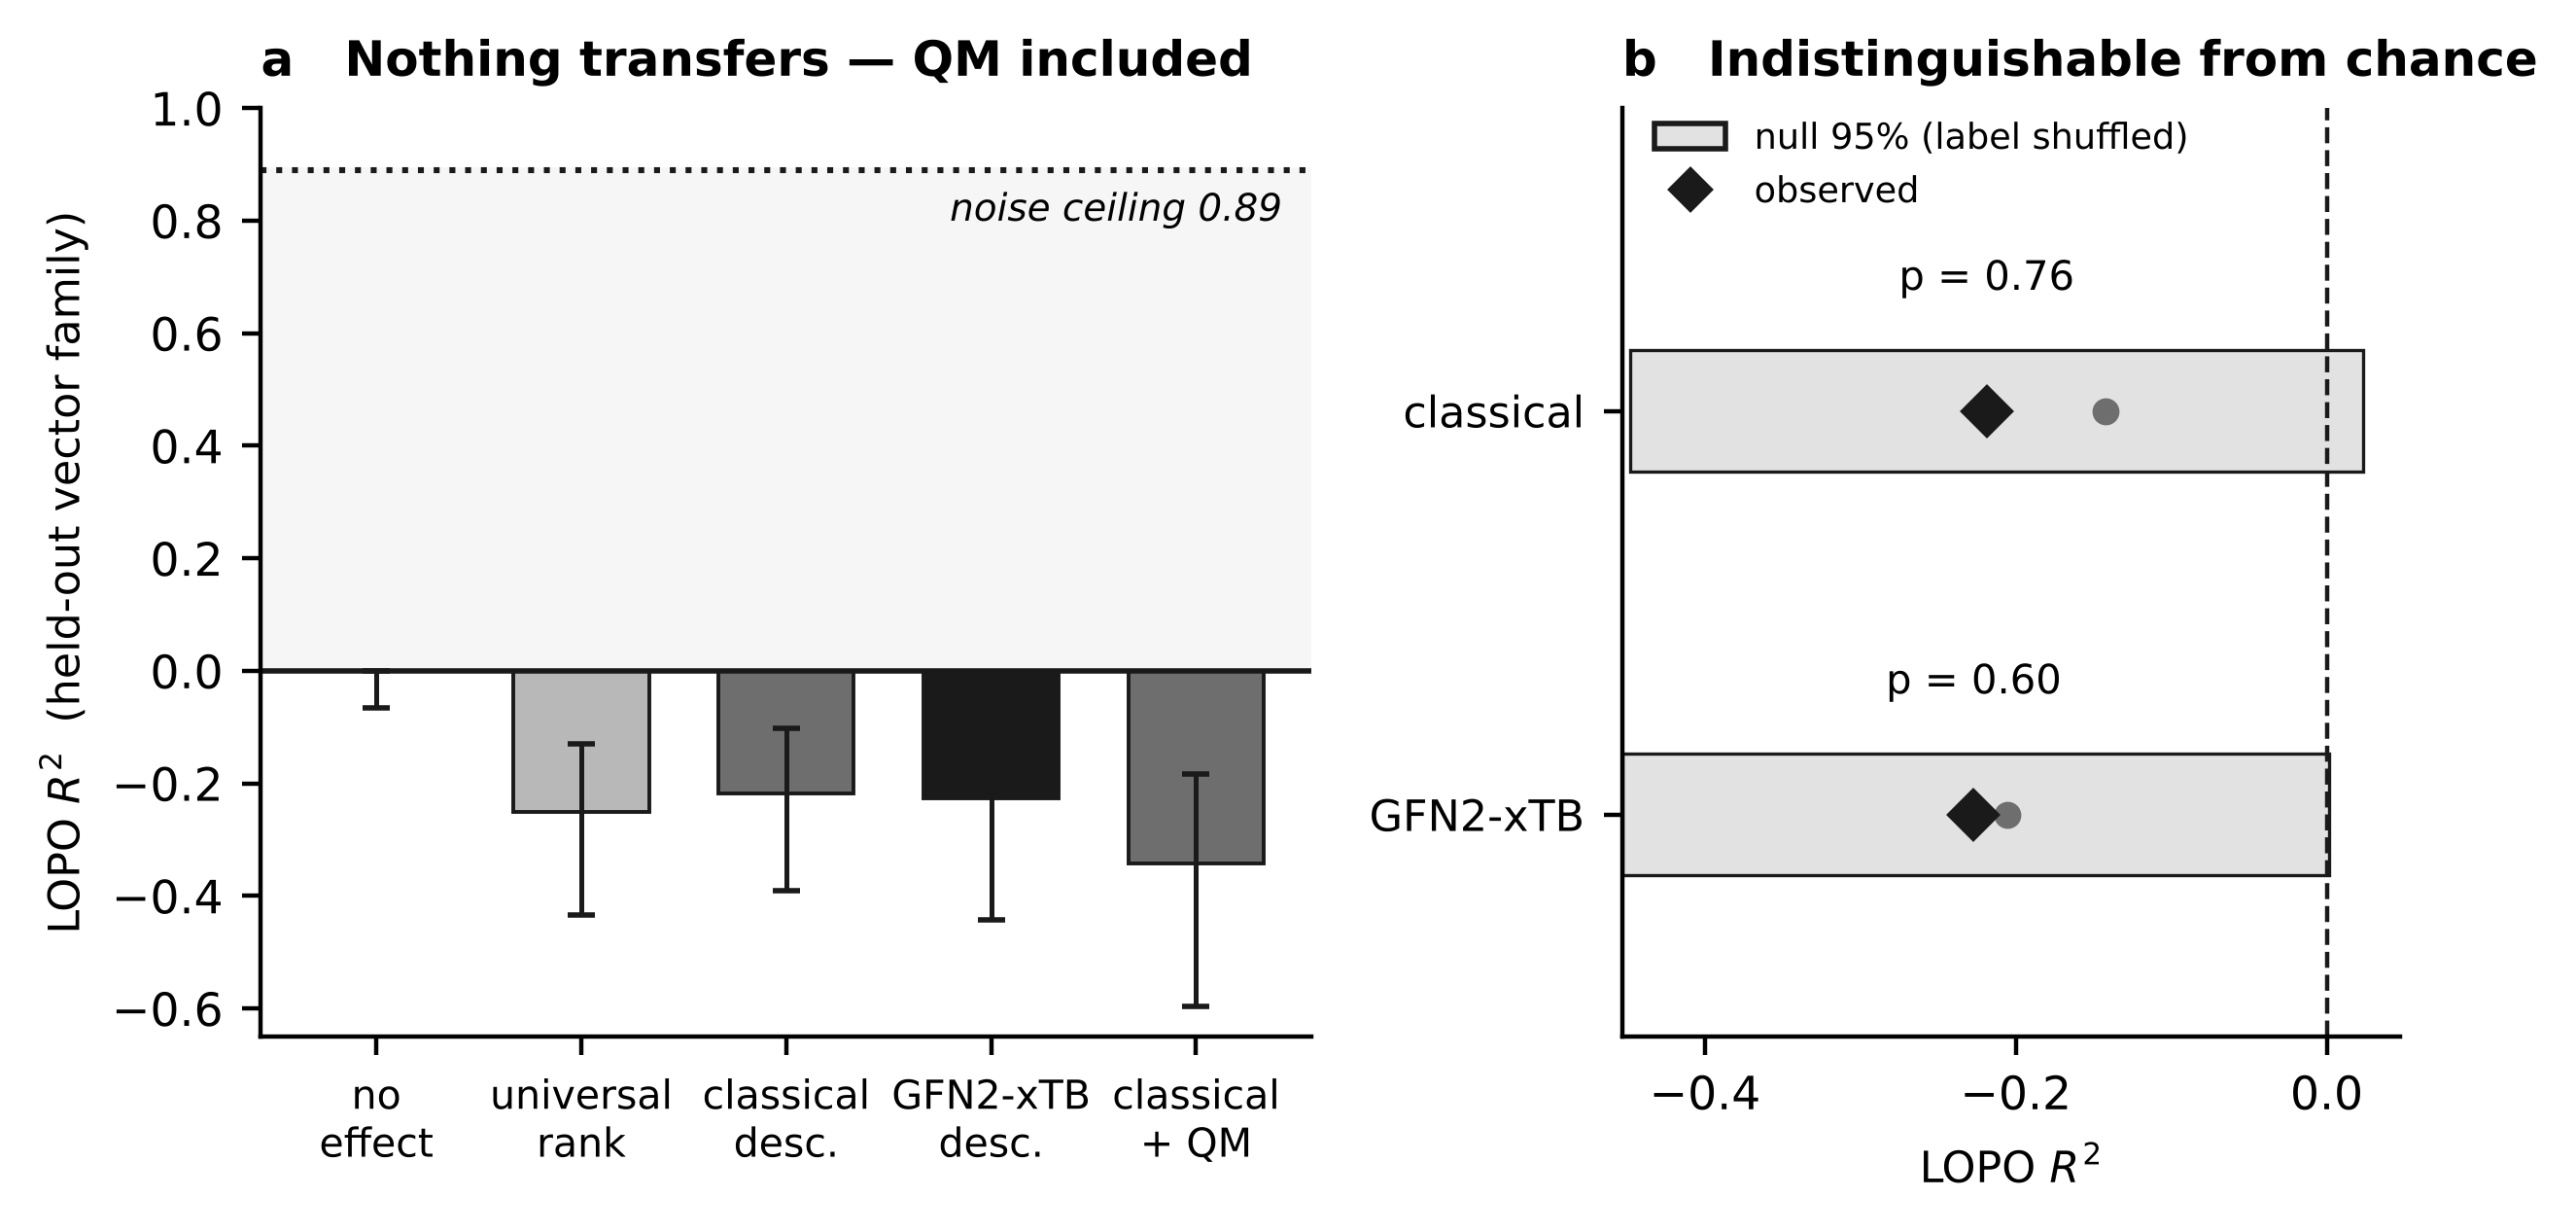
\includegraphics[width=\columnwidth]{Fig2.png}
\caption{\textbf{No descriptor set transfers to a held-out target family.} (\textbf{a}) Leave-one-target-family-out $R^2$ for five models ($n = 82$); error bars, 10\,000-sample bootstrap 95\% CI; shaded region, the range up to the measurement-noise ceiling of 0.890. (\textbf{b}) Observed LOPO $R^2$ (diamonds) against the null distribution from 2000 within-set label permutations (boxes, 95\% interval; circles, null mean).}
\label{fig:2}
\end{figure}

\begin{figure}[t]
\centering
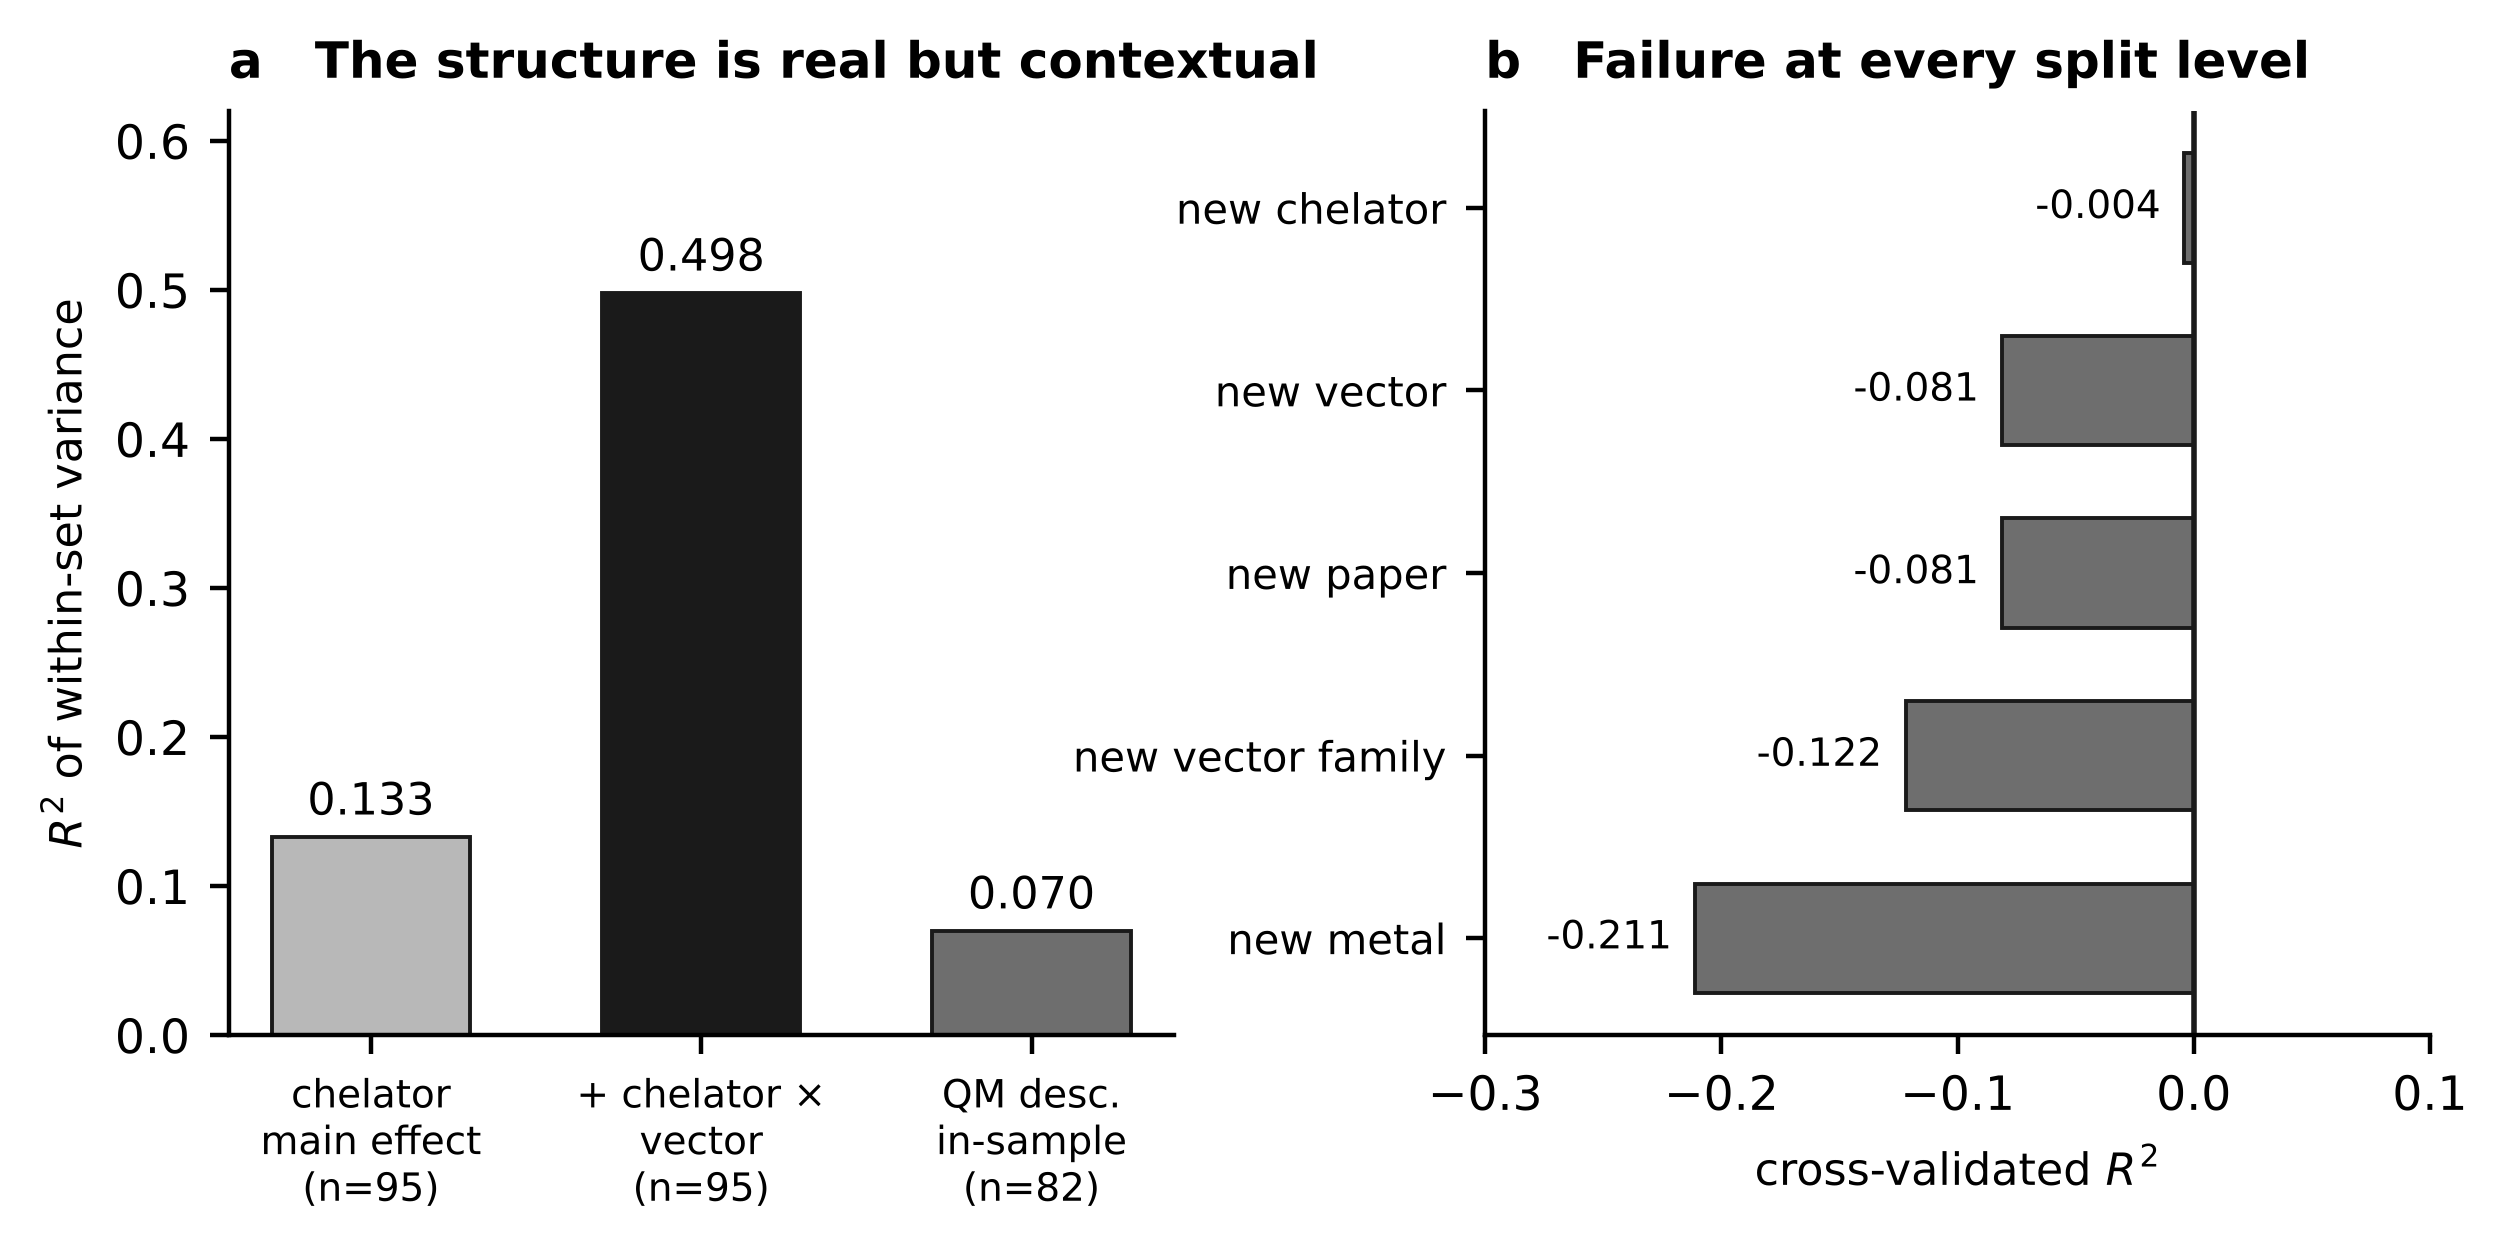
\includegraphics[width=\columnwidth]{Fig3.png}
\caption{\textbf{The effect is structured but contextual, and transfer fails at every level.} (\textbf{a}) Fraction of within-set variance explained by chelator alone and by chelator interacted with target family (full 95-row set), and by quantum-chemical descriptors fitted in sample (82-row subset). (\textbf{b}) Cross-validated $R^2$ under five held-out grouping schemes.}
\label{fig:3}
\end{figure}

\begin{figure*}[t]
\centering
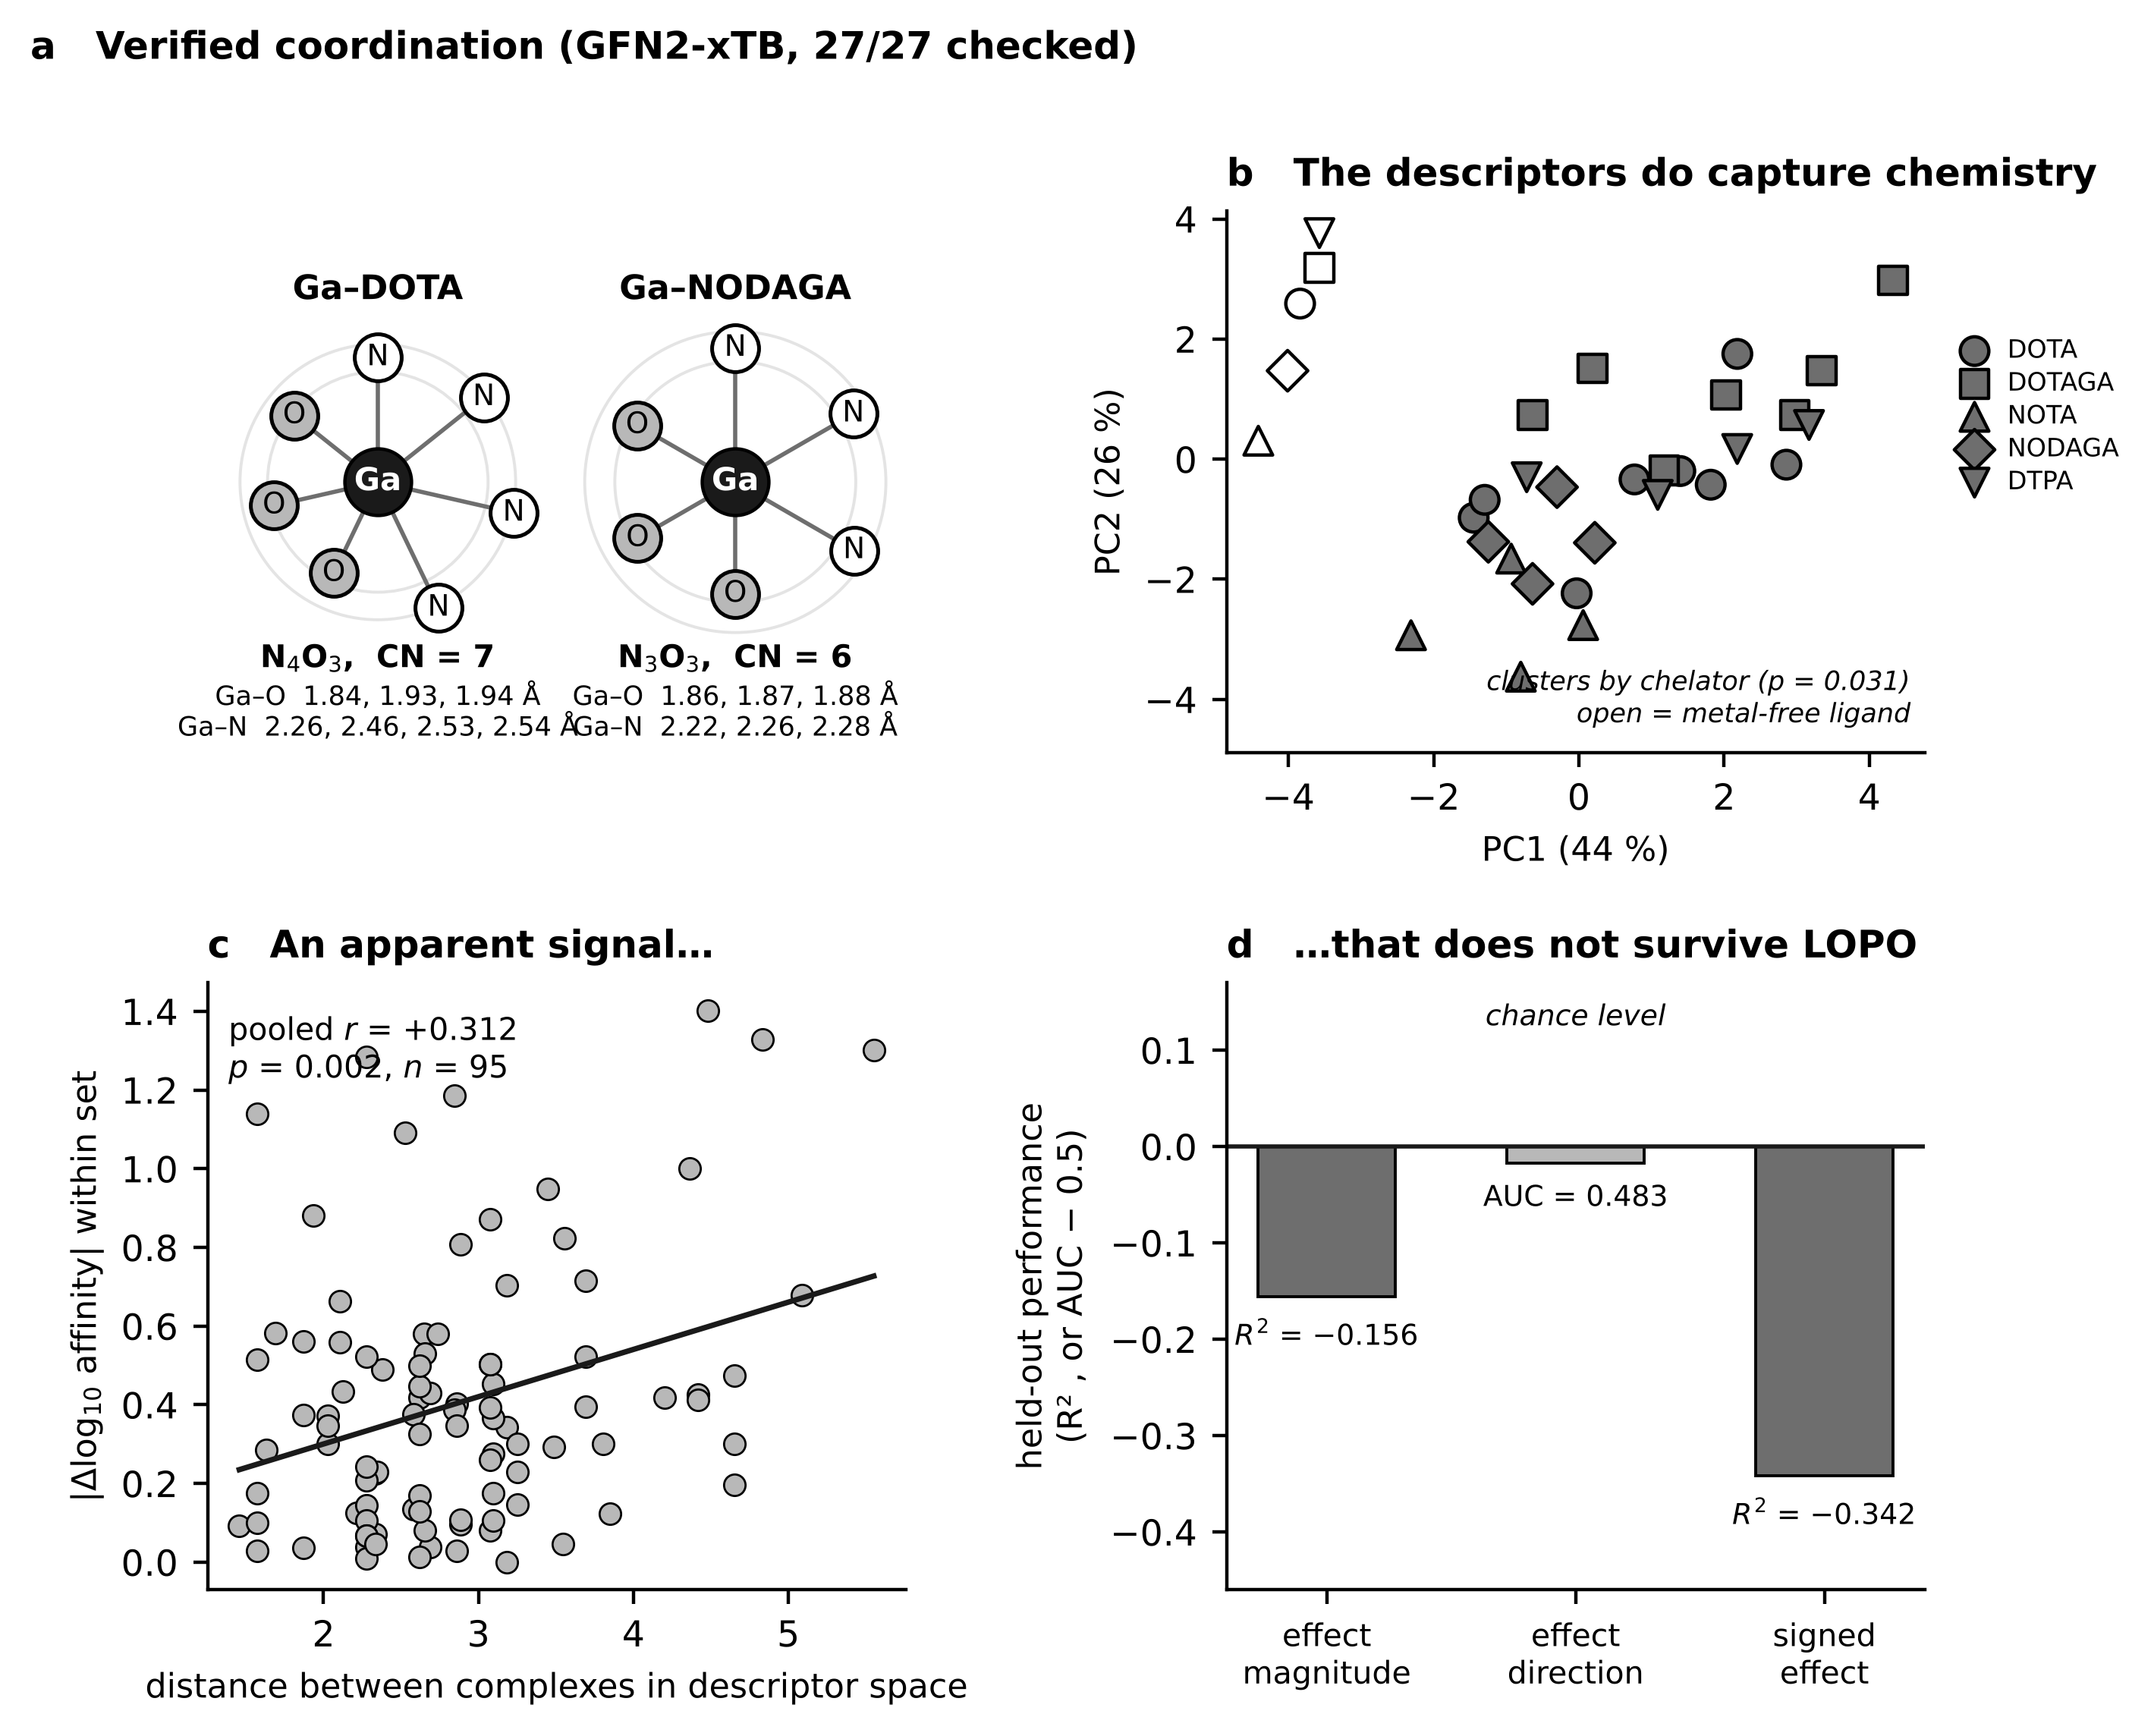
\includegraphics[width=0.86\textwidth]{Fig4.png}
\caption{\textbf{The descriptors are chemically sound, and the signal they appear to carry does not survive held-out validation.} (\textbf{a}) Coordination fingerprints of two optimised complexes, Ga--DOTA and Ga--NODAGA; donor atoms are placed at equal angles with the radius equal to the computed metal--donor distance. Coordination mode was verified against the known mode for every complex (27/27). (\textbf{b}) The 32 complexes in the first two principal components of the twelve descriptors; symbols denote chelator, open symbols the metal-free ligand. (\textbf{c}) Distance between two complexes in descriptor space against the magnitude of the affinity difference between them, pooled over all 95 within-set chelator pairs. (\textbf{d}) The same quantities under leave-one-target-family-out validation: magnitude, direction and the signed effect. Direction is shown as AUC $-$ 0.5 on the same axis and was evaluated on the antisymmetrised pair set, so that zero on this axis is chance by construction.}
\label{fig:4}
\end{figure*}

%%============================================================
\section{Methods}
%%============================================================

\subsection{Study identification and matched-set extraction}

Ten seed papers comparing chelators on a common vector were expanded through their Semantic Scholar citation and reference networks, yielding 681 unique DOIs. Titles and abstracts were screened for two or more distinct chelators from a controlled vocabulary of 28 chelator cores, a measured affinity endpoint, a targeting vector, and comparison language, giving 42 candidate studies of which 38 (90\%) were open access. Full texts were retrieved as structured XML through the Europe PMC REST API.

Affinity tables were read and transcribed by hand; no value was obtained by automated parsing, interpolation or estimation. Each record carries its source DOI, vector, chelator, metal, endpoint, value, standard deviation and a provenance note. Values that a source reproduced from earlier work were identified by their footnotes and excluded as duplicates---three pentixafor studies\cite{Poschenrieder2016a,Poschenrieder2016b,Poschenrieder2017} share one underlying dataset.

The analysis unit is the \emph{matched set}: one paper, one vector, one metal, one endpoint, with the chelator varying, so that assay, cell line, radioligand and vector are constant. The final dataset comprises 106 values from ten studies,\cite{Poschenrieder2016a,Poschenrieder2017,Mitran2019,Fischer2025,Weineisen2014,Sinnes2020,Basaco2024a,Basaco2024b,Rinne2019,Rinne2020} of which 95 fall in 32 matched sets spanning five target families (CXCR4, GRPR, PSMA, SSTR, affibody/DARPin), 13 vectors, nine chelators and ten metal states. Endpoints were IC$_{50}$ (71), $K_\text{D}$ (18) and $K_\text{i}$ (6); set sizes ranged from two to eight chelator arms. Values were log$_{10}$-transformed and centred within their matched set.

\subsection{Descriptors}

\emph{Classical (10).} Net formal charge of the metal--chelate unit in the conjugated form (one arm consumed by the amide bond to the vector), number of free carboxylates, macrocycle nitrogen count and ring size, denticity, macrocyclic flag, metal formal charge, Shannon ionic radius, a metal-present flag, and a cavity-fit mismatch term.

\emph{Quantum-chemical (12).} For every (chelator, metal) combination in the dataset the conjugated ligand was built from SMILES with one arm capped as an $N$-methylamide, the metal threaded into the cavity using explicit dative bonds before 3-D embedding, and the complex relaxed with GFN2-xTB\cite{Bannwarth2019,Bannwarth2020} at the correct total charge and spin with the ALPB implicit solvation model\cite{Ehlert2021ALPB} in water. These are charged species---the conjugated complexes carry formal charges from $-4$ to $+1$---and a gas-phase treatment of them is not defensible. Five starting structures were used per complex (four fresh conformer seeds plus a re-relaxation of a gas-phase optimum) and the lowest-energy structure with a chemically valid coordination mode kept. This is a deliberately modest conformer search by the standards of dedicated samplers,\cite{Pracht2024CREST} and we verified that it was sufficient by the coordination-mode check described below rather than by energy convergence alone.

Complexation energies referenced to the bare metal ion are dominated by Coulombic neutralisation rather than chemistry: computed that way they span $-691$ to $-2257$\,kcal\,mol$^{-1}$ and correlate with the metal's formal charge at $r = -0.914$, and implicit solvation alone does not repair this ($r = -0.884$). We therefore used a \emph{ligand-exchange energy} referenced to DOTA at the same metal, $\Delta\Delta E(\mathrm{L};\mathrm{M}) = [E(\mathrm{ML}) - E(\mathrm{L})] - [E(\mathrm{M}\cdot\mathrm{DOTA}) - E(\mathrm{DOTA})]$, in which the ion term cancels exactly. It spans $-35.7$ to $+20.6$\,kcal\,mol$^{-1}$ and its correlation with metal charge falls to $r = -0.199$ ($p = 0.320$).

Coordination geometry was verified against the known coordination mode of each chelator rather than assumed, giving 27/27 verified complexes (Ga--DOTA N$_4$O$_3$ with Ga--O 1.84--1.94\,\AA{} and Ga--N 2.26--2.54\,\AA; Ga--NODAGA N$_3$O$_3$; Lu--DOTA N$_4$O$_4$). Solvation changed the structures materially---four of 27 coordination numbers shifted, mean M--N contracted by 0.10\,\AA, and the mean dipole moment rose from 16.0 to 25.9\,D.

Every log$D_{7.4}$ or log$P$ value reported alongside the affinity data in the same tables (38 values from four of the ten studies) was transcribed and tested as a confounder.

\subsection{Models and validation}

All models predicted the within-set deviation. Comparators were: predicting zero; a one-hot chelator encoding, which is the model implied by a universal chelator ranking; classical descriptors; and quantum-chemical descriptors, alone and combined. Continuous features were standardised and fitted with ridge regression.

Validation was leave-one-target-family-out. Random splits are invalid here: matched sets contribute several rows sharing a vector, so a random split places one arm of a construct in training and another in test, leaking the set mean---the mechanism by which random splits inflate reported performance on structurally clustered chemical data.\cite{Kim2026TAS2R,Boldini2025UMAP,Tropsha2025Eval} Transfer was additionally evaluated with held-out chelator, vector, paper and metal. Confidence intervals come from 10\,000 bootstrap resamples and ten random seeds were averaged. A within-set label-permutation test (2000 permutations) provides the null distribution of LOPO $R^2$ under no transferable information. Normality was assessed by Shapiro--Wilk ($W = 0.982$, $p = 0.233$); paired contrasts used Wilcoxon signed-rank with Cohen's $d_z$.

Pairwise analyses (Fig.~\ref{fig:4}c,d) were computed on all 95 within-set chelator pairs, with distances taken in the standardised descriptor space. Because the ordering of the two members of a pair is arbitrary, the signed quantities were evaluated on the antisymmetrised pair set---each pair entered twice with the sign of both the label and the descriptor difference reversed---so that chance performance on direction is exactly 0.500 by construction rather than by assumption. The two axes of physical improvement (energy term and solvation) were evaluated as a full $2 \times 2$ on the same 82 rows.

Three pre-specified sanity checks were applied before interpretation---monotonicity of the response against complex charge, correctness of the within-set centring, and consistency between the IC$_{50}$-only subset and the full set. All three passed ($\rho = -0.208$, $p = 0.043$ in the hypothesised direction; maximum absolute within-set mean $1.7\times10^{-16}$; IC$_{50}$-only $\rho = -0.243$).

%%============================================================
\section*{Conflicts of interest}
%%============================================================
There are no conflicts to declare.

%%============================================================
\section*{Data availability}
%%============================================================
The data supporting this article are available in full. The matched affinity dataset with per-row DOI provenance, the derived analysis table, the quantum-chemical descriptors and optimised Cartesian geometries of all 32 metal--chelate complexes, the screened candidate pool and the complete analysis pipeline are archived at Zenodo under CC-BY-4.0 (DOI: \texttt{10.5281/zenodo.24211564}), with development history at \url{https://github.com/bisu9082/chelfit}. Every affinity value was transcribed by hand from an open-access full text and carries its source DOI; no value was parsed automatically, interpolated, estimated or generated. Running the pipeline from the deposited files reproduces every number and figure in this article.

%%============================================================
\section*{Author contributions}
%%============================================================
J.K. and J.Y. contributed equally. J.K.: quantum-chemical calculations, methodology, validation, writing---review and editing. J.Y.: data curation, investigation, validation, writing---review and editing. K.K.: conceptualization, formal analysis, methodology, software, visualization, writing---original draft, supervision. D.L.: conceptualization, interpretation, writing---review and editing, supervision. All authors approved the final manuscript. [Per-author allocation to be confirmed by the co-authors before submission.]

%%============================================================
\section*{Acknowledgements}
%%============================================================
[To be completed.]

%%============================================================
\balance
\renewcommand\refname{Notes and references}
\bibliographystyle{rsc}
\bibliography{references}

\end{document}
